
\chapter{Data collection and processing}
\label{chap:methods}

% NC: In general here be careful not to go overboard with details. I've tried to make it a bit more concise. We don't want your poor examiner to expire with the weight of the thesis esp as it's already 40 pages without the main chapter!!!

\section{Introduction} % NC: Perhaps "Overview" rather than introduction?

	I compiled a morphological data set of both photographs and linear measurements from 366 specimens representing 99 species of small mammals. 
	%(total number of skulls and species in Access Data base, excluding the two _sp.)
	I collected morphological data from skulls, limbs and skins. 
    
    % NC: I think just mention this in the discussion and don't draw attention to it here
	%However, for this thesis, I have only analysed a subset of the skull data (chapter \ref{chap:disparity}). Therefore my linear measurements of skulls and limbs along with photographic record of skins represent significant data sources for future work. 
	%put in reference to the future work section in the last chapter 
	
	I have divided my description of how the data were collected and analysed % NC: Do you mean analysed or processed? I think we want a distinction between the disparity analyses and the Procrustes etc which is really post data collection data processing.
	into three sections:
	
	\begin{enumerate}[i]
	
	\item Data collection (section \ref{sect:datacollection}): \\
	Summary of the species measured, information recorded from museum labels, linear measurements and photographic set up.
	
	\item Geometric morphometric analyses (section \ref{sect:morphometrics}):\\
	Landmark and semilandmark placement on different views of skulls and mandibles.
	
	\item Error checking (section \ref{sect:errors}): \\
	How I dealt with errors in taxonomic and specimen identification, possible variation associated with sex and age class, accuracy and repeatability of linear measurements and morphometric errors associated with photographing specimens and the placement of landmarks.
	
% NC: Add item for supp methods 
%\item Additional data collection. Much of the data I collected was not necessary for the projects in this thesis so I have documented the collection of this data in ???
	
	\end{enumerate} 


%####################################################
\section{Data collection}
\label{sect:datacollection}
%##################################################


\subsection{\normalfont{Species measured and taxonomy}}

	Between January and September 2013, I spent a total of 9 weeks working in the collections of five museums: the Natural History Museum, London (BMNH), the Smithsonian Institute Natural History Museum, Washington D.C. (SI), the American Museum of Natural History, New York (AMNH), Museum of Comparative Zoology, Cambridge (MCZ) and the Field Museum of Natural History, Chicago (FMNH). I measured and photographed 366 skulls, 248 post-cranial skeletons and 277 skins from 101 species belonging to four mammalian Orders: Afrosoricida, Erinaceomorpha, Soricomorpha and Notoryctemorphia. These belonged to seven families of mammals: tenrecs (Tenrecidae), golden moles (Chrysochloridae), hedgehogs and gymnures (Erinaceidae), shrews (Soricidae), solenodons (Solenodontidae), moles and desmans (Talpidae) and marsupial moles (Notoryctidae).

	% NC: I would instead say belonging to seven families within four orders, then group the families within their orders to make it clearer.

	I measured all the tenrecs and golden moles available in the collections (31 species of tenrec, 12 species of golden moles, table \ref{tab:species.measured}). % NC: Out of how many species?
	For my comparative species of non-Afrosoricida species, I chose a random sample of 56 taxa 
	%non tenrec or golden mole species in the Access data base 
	which have been previously identified as convergent with tenrecs \citep[e.g.][]{Gould1966, Symonds2005, Poux2008, Olson2013}. 
% NC: I don't understand the paragraph below. Might be better to mention the taxonomy used somehwere else. Especially as you've already been using in the paragraphs above...The phylogeny is actually the bininda emonds tree right?
	Following the taxonomy in Wilson and Reeder's Mammal Species of the World (MSW) \citeyearpar{Wilson2005}, I used phylogenies for each Order to select species at random which represented the main sub-branches and morphological diversity of each Order. For example, within the Soricomorpha, I only included three %number of Crocidura species in Access data base
	species of \textit{Crocidura} (out of a total of 230, Wilson and Reeder \citeyear{Wilson2005}) but both species of \textit{Solenodon} because it represents a separate subgroup to the rest of the Order. 

	I used the taxonomy of Wilson and Reeder's Mammal Species of the World \citeyearpar[MSW,][]{Wilson2005} supplemented with more recent sources \citep[e.g.][]{Olson2013, Soarimalala2011} to identify the specimens. % NC: Well you didn't use it to identify them as such. You used it to define their names... Rephrase
	Table \ref{tab:species.measured} outlines the number of species I measured from each Family and how this sample relates to the overall number of species in that group as recorded in MSW \citeyearpar{Wilson2005}. % NC: I'd write Mammal Species of the World not the abbreviation.

%####################################################
%Species.measured table

% NC: Really this is meant to show the % you measured of what you count as species. So the MSW total should really be MSW plus additional stuff for tenrecs at least. Also add a % coverage column so it's easier to see coverage.

\begin{table}[h]
	\caption[Species measured] 
	{The number of species measured in each Family compared to the total number of species in that Family according to Mammal Species of the World version 3 \citeyear{Wilson2005} (MSW).}
	%Species.measured table
%To get the number measured for each Family, I counted the number of unique species in my Tb_Taxonomy Access table for that family
%So it's the number of species measured overall but that doesn't necessarily mean that I have the same number in every data set
%I didn't count the _sp. specimens as separate species

%I took out the reference to the IUCN because it seems to only list species that are threatened/endangered rather than a full list of all species in a family

\begin{tabular}{p{3.4cm}p{3cm}p{2cm}p{2cm}p{2cm}}

\hline
\textbf{Order} & \textbf{Family} & \textbf{Measured species} & \textbf{Total species} & \textbf{Coverage} \\
\hline
%----------------------------------------------------
Afrosoricida & Tenrecidae & 31 & 34 & 91 \% \\
%-------------------------------------------------
Afrosoricida & Chrysochloridae & 12 & 21 & 57 \% \\
%----------------------------------------------------
Erinaceomorpha & Erinaceidae & 16 & 24 & 67 \% \\
%----------------------------------------------------
Soricomorpha & Soricidae & 22 & 376 & 5.8 \% \\
%----------------------------------------------------
Soricomorpha & Solenodontidae & 2 & 4 & 50 \% \\
%----------------------------------------------------
Soricomorpha & Talpidae & 15 & 39 & 38 \% \\
%----------------------------------------------------
Notoryctemorphia & Notoryctidae & 1 & 2 & 50 \% \\
%-----------------------------------------------
\hline

\end{tabular}

%*There are now 34 recognised tenrec species \citep{Olson2013}	
	\label{tab:species.measured}
\end{table}
 
%####################################################
Wilson and Reader \citeyearpar{Wilson2005} record 30 species of tenrec but more recent studies indicate that there are now 34 species\citep{Olson2013}. The additional species belong to the shrew tenrec (\textit{Microgale}) Genus and represent either recognition of cryptic species boundaries \citep{Olson2004} or discovery of new species \citep{Goodman2006, Olson2009}. Only one of these four recent additions, \textit{M. jobihely}, was present in the museum collections and therefore I could not include the three other newly recognised species in my analyses.


%------------------------------------------------------


\subsection{\normalfont{Museum label data}} % NC: Or are they more correctly specimen labels?

	I recorded all the data on the specimen labels including any handwritten or printed notes which had been added by other users of the collection. The label data included the museum specimen accession number, Genus, species, sex, collector's name, and the date and location of collection. Some of the labels attached to skins had additional information such as the body, tail, hind foot and ear lengths as well as the body mass of the live individual. 
	
	%The level of detail recorded on the labels varied considerably (figure \ref{fig:museum.labels}). For example, recently collected specimens were more likely to have detailed information about the collection location whereas some specimens did not have even basic information such as the sex recorded. % NC: True, but is this relevant? Not really I think.

%Museum label pictures % NC: Again not really relevant

%\begin{figure}[h] 
 % \centering
  %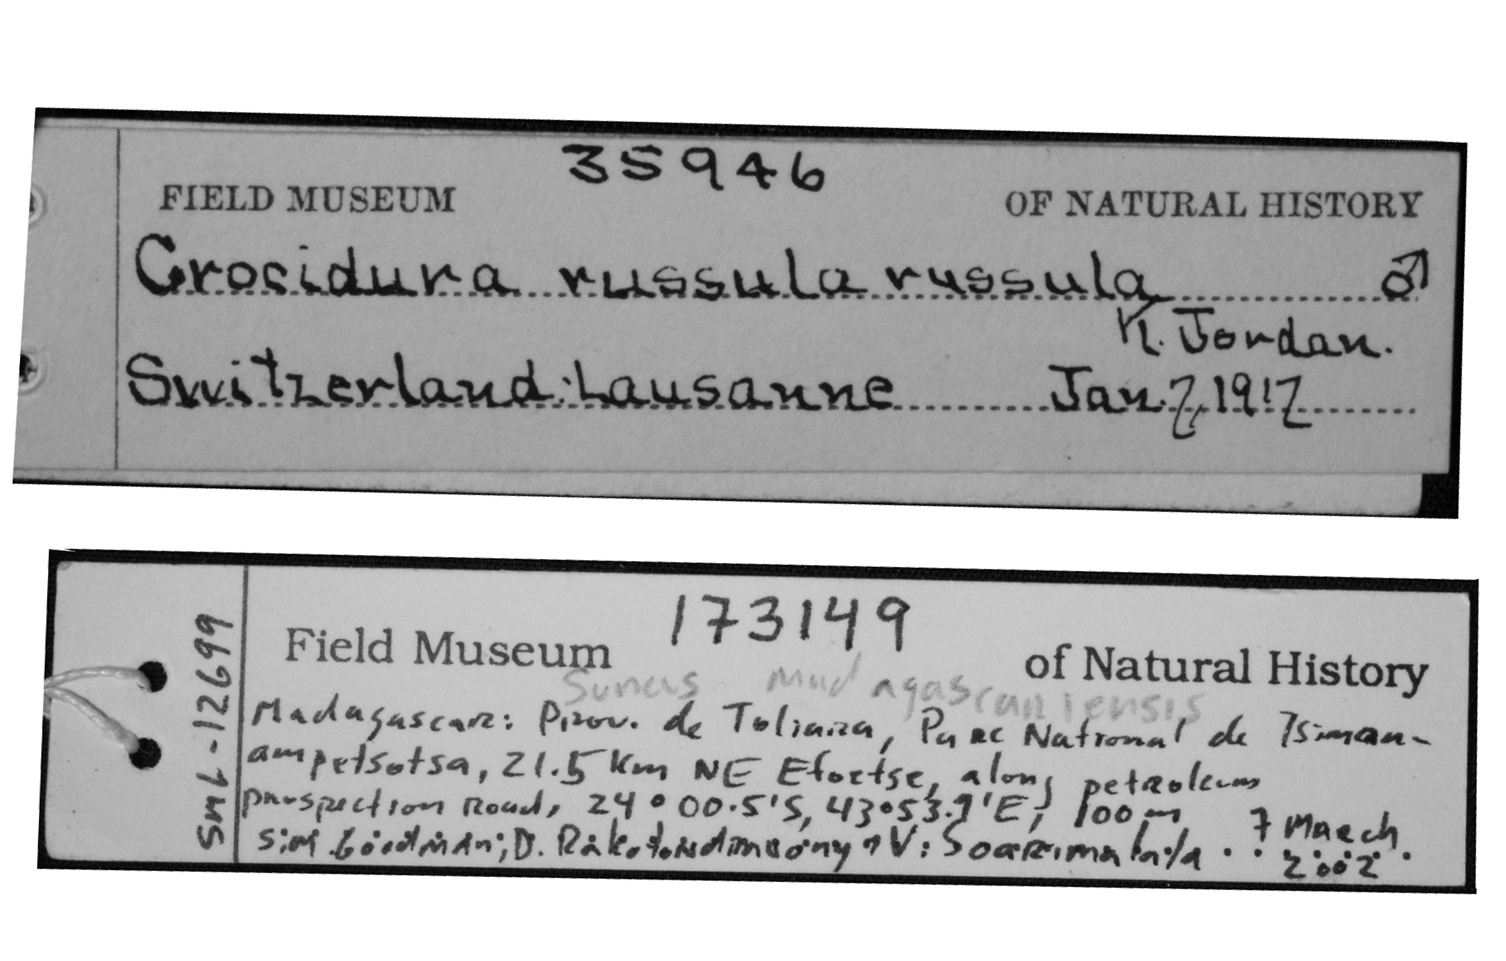
\includegraphics[width = 15cm, height = 15cm, keepaspectratio=true]{Methods/figures/labels.png}
   % \caption[Examples of museum labels]
    %{Examples of the variation in the detail of information which is available from museum labels.}
  %\label{fig:museum.labels}
%\end{figure}
  
%------------------------------------------------
\subsection{\normalfont{Linear measurements}} 
\label{sect:measurements} %Label the section so I can refer to it in the error checking later on

	Using 15 mm digital calipers (Mitutoyo Absolute digimatic calipers), I took five measurements from each mandible (table \ref{tab:mands.measurements}), 15 from each skull (table \ref{tab:sk.measurements}) and 19 from each set of limbs (table \ref{tab:limb.measurements}). My choice of  measurements was based on three main criteria; 1) their relevance to biological and ecological traits such as diet specialisation and locomotory adaptation; 2) their usefulness for assessing the overall shape and size of the specimen; and 3) the ease with which they could be repeated both within and among specimens from different species. 
	%Figures x-x depict the linear measurements of skulls and figures xx show the limb measurements.
	%Maybe I could get away with no pictures?
	%It would be tricky to show all of the measurements on single images

	% NC: Depends. If you ever want people to be able to sue this data then pictures are necessary aren't they? However, you could just cut all the linear measurement stuff as you don't use it at all. I'd be tempted to do this because your thesis is already huge! You could pop this all into supplementary.

	I took each linear measurement three times, cycling through all 20 skull or 19 limb measurements then repeating the cycle to avoid measuring the same variable twice in a row. Small measurements (<2 mm) are particularly prone to high error rates \citep{Cardini2008}. Therefore, I took five separate replicates of some of the measurements which were often less than 2 mm and consequently most prone to errors (marked with * in tables \ref{tab:sk.measurements} and \ref{tab:limb.measurements}). These included four of the skull measurements (PWa, IncisorH, IFD and IFcanal, table \ref{tab:mands.measurements}) and five of the limb measurements (FemD, TibD, HumD, UlnD, RadD, table \ref{tab:limb.measurements}). 
	Five replicates should give a more reliable median value because even if there are one or two outlying measurements there should be at least three replicates which are in close agreement \citep{Cooper2009}.
	
	%Could put in an explanation of why there are extra measurements for golden mole limbs and why I used minimum diameter of the bones - loading capacity

%******************************
%The tables are very long so maybe I should stick them into an appendix or give shorter descriptions of the measurements?

% NC: No leave them here or the rest of the methods get hard to understand. 3 pages is fine. Also can you please sort out the widths of the last column. I showed you how to do it before.

% Mandible  measurements

\begin{table}[!htbp]
	\caption[Mandible measurements]
			{Measurement abbreviations and descriptions for the mandibles, all taken from the labial (outer) side of the right jaw unless that side was broken or missing. All measurements were repeated three times except for those marked with * which were measured five times.}
	%Mandible measurements

\begin{tabular}{p{2.5cm}p{3.2cm}p{7.5cm}}
\hline
\textbf{Abbreviation} & \textbf{Measurement} & \textbf{Description}\\
\hline
ML & Mandible length & Maximum jaw length measured from the symphysis to the end of the jaw in a straight line to the condyloid crest/posterior notch\\
%-------------------------------------------
MTR & Mandible tooth row length & Anterior edge of the alveolus of the first tooth to the posterior edge of the alveolus of the last tooth on the same side\\
%----------------------------------------------
CorP & Coronoid process height & Perpendicular height from the top of the coronoid process to the base of the jaw bone\\
%----------------------------------------------
ConY & Condyloid height & Perpendicular height from the top of the mandibular condyle to the base of the jaw\\
%----------------------------------------
CorCon & Coronoid-condyloid length & Diagonal distance from the coronoid tip to the condyloid crest/posterior notch \citep{Carraway1996}\\
%--------------------------------------------
\hline
\end{tabular}
	\label{tab:mands.measurements}
\end{table}

%Skull measurements
\begin{table}[!htbp]
	\caption[Skull measurements]
			{Measurement abbreviations and descriptions for the skulls. All measurements were repeated three times except for those marked with * which were measured five times.}% add to this caption
	%Skull measurements

\begin{tabular}{lp{3.5cm}p{9.75cm}}
\hline
\textbf{Abbreviation} & \textbf{Measurement} & \textbf{Description}\\
\hline
CB & Condylobasal length & Total skull length from the front of the premaxillary  bones to the rear of the occipital condyles, measured from below \\
%-------------------------------------------
PL & Palate length & Maximum length of the palate from the anterior of the pre-maxilla to the posterior of the hard palate\\
%----------------------------------------------
TR & Tooth row length & From the front of the alveolus of the first incisor to the rear of the alveolus of the last molar on the same side\\
%----------------------------------------------
PWa* & Palate width anterior & Width across the palate measured between the posterior, outer-most points of the alveoli of the first pair of teeth\\
%I had to modify this measurement slightly for some species: when there was a row of anterior incisors which stretch across the front of the palate (e.g. Euroscaptor klossi SI_261090) then I measured PWa as the width across from back of the row of the incisors on either side (i.e. just in front of the canines) 
%----------------------------------------
maxPW & Maximum palate width & Measured at the widest point of the palate\\
%--------------------------------------------
IncisorH* & Incisor height & Maximum height of the first incisor on the right\\
%----------------------------------------
ZW & Zygomatic width & Maximum width between the zygomatic arches (measured within the arches from below the skull)\\
%---------------------------------------
MX & Maxilla width & Width between the maxillary bones, measured from above the skull. Species with zygomatic arches; width from the innermost connection between the anterior of the arch and the skull. No arches; width between the anterior skull constrictions.\\ 
%---------------------------------------
SQ & Squamosal width & Width between the squamosal bones, measured from above the skull. Species with zygomatic arches; width from the innermost connection between the posterior of the arch and the skull. No arches; width between the posterior skull constrictions \\
%-------------------------
OL & Orbit length & Longitudinal length of the orbit opening measured along the edge of the skull from the maxilla to the squamosal. \\
%------------------------------
IFD* & Interorbital foramen width & The maximum (vertical) diameter of the right interorbital foramen\\
%-----------------------------------------------
IFW & Interorbital foramen width & Maximum width across the skull between the two interorbital foramina, measured from above\\
%-------------------------------
IFcanal* & Interorbital foramen canal & Length of the right IF canal measured between the anterior and posterior openings from above\\
%---------------------------------
BW & Braincase width & Width across the braincase at the widest point of the skull\\
%---------------------------------
SkH & Skull height & Perpendicular height from the highest point on the braincase to the base of the skull\\



\hline
\end{tabular}
	\label{tab:sk.measurements}
\end{table}



% Limb measurements
\begin{table}[!htbp]
	\caption[Limb measurements]
		{Measurement abbreviations and descriptions for the limbs. All measurements were repeated three times except for those marked with * which were measured five times.} % add to this caption
	%Limb measurements


\begin{tabular}{lp{3.5cm}p{9.75cm}}
\hline
\textbf{Abbreviation} & \textbf{Measurement} & \textbf{Description}\\
\hline
Inn & Innominate length & Maximum longitudinal length of the pelvic bone measured in a straight line from the anterior tip to the posterior curve \\ 
%-----------------------------------
Obt & Obturator foramen & Maximum diameter of the opening in the pelvic bone \\
%-----------------------------------
FemL & Femur length & Length of the bone excluding the femoral head (i.e. length of the bone without the joint area)  \\
%-----------------------------------
FemD* & Femur diameter & Minimum width across the shaft of the bone \\
%-----------------------------------
TibL & Tibia length & Maximum longitudinal length of the tibia  \\
%-----------------------------------
TibU & Tibia unfused length & Length of the tibula which is not fused with the fibula \\
%-----------------------------------
TibD* & Tibia diameter & Minimum diameter across the shaft of the tibia bone \\
%-----------------------------------
Foot & Foot length & Maximum length of the entire foot (heel to longest toe) \\
%-----------------------------------
Toe & Toe length & Length of the longest toe bone (just the phalange bone up to the metatarsal joint) \\
%-----------------------------------
ScapL & Scapula length & Perpendicular length of the scapula from the curved end to the anterior point  \\
%-----------------------------------
ScapW & Scapula width & Maximum perpendicular width across the bone \\
%--------------------------------
HumL & Humerus length & Maximum length of the bone. In golden moles (L-shaped humerus): diagonal distance between the two ends of the bone  \\
%-------------------------------
HumLvert & Humerus length vertical & Only for golden moles with L-shaped humerus: length of the vertical (longer) side of the bone \\
%-------------------------------
HumLhori & Humerus length horizontal & Only for golden moles with L-shaped humerus: length of the horizontal (shorter) side of the bone \\
%-----------------------------------
HumD* & Humerus diameter & Minimum diameter across the shaft of the humerus \\
%-----------------------------------
UlnL & Ulna length & Length of the bone from the posterior tip to the wrist joint \\
%-----------------------------------
RadL & Radius length & Length of the bone from the posterior tip to the wrist \\
%--------------------------------
UlnD* & Ulna diameter & Minimum diameter across the ulna \\
%-------------------------------
RadD* & Radius diameter & Minimum diameter across the radius \\
%----------------------------
Hand & Hand length & Maximum length of the entire hand (wrist to longest finger) \\
%------------------------
Finger & Finger length & Length of the longest finger bone (to the metatarsal joint) \\
%---------------------
\hline

\end{tabular}
	\label{tab:limb.measurements}
\end{table}


%****************************
%####################################################
\newpage
\subsection{\normalfont{Photographic set up}}

% NC: Be consistent: are they photographs or pictures? Throughout you chop and change at random


	In order to get 2D landmarks for my specimens, I first had to photograph them. I used photographic copy stands consisting of a camera attachment with an adjustable height bar, a flat stage on which to place the specimen and an adjustable light source. To take possible light variability into account, on each day I took a picture of a white sheet of paper and used the custom white balance function on the camera to set the image as the baseline "white" measurement for those particular light conditions.
	
	I photographed the specimens with a Canon EOS 650D camera fitted with either an EF 100 mm f/2.8 Macro USM lens (skulls and limbs) or EFS 18-55 mm lens (skins). I used a remote control (h\"ahnel Combi TF) to take the photos to avoid shaking the camera and distorting the images. I photographed the specimens on a black material background. I placed the light source from the top left-hand corner of the picture and positioned a piece of white card on the bottom right side of the specimen which reflected the light back onto the specimen and minimised any shadows (figure \ref{fig:camera}). I used small bean bags as necessary to hold the specimens in position while being photographed to ensure that the specimen I was photographing lay in a flat plane relative to the camera and did not tilt in any direction. I used the grid-line function on the live-view display screen of the camera to position the specimens in the centre of each image. 

%----------------------------------------------
%Camera picture
\begin{figure}[h] 
  \centering
  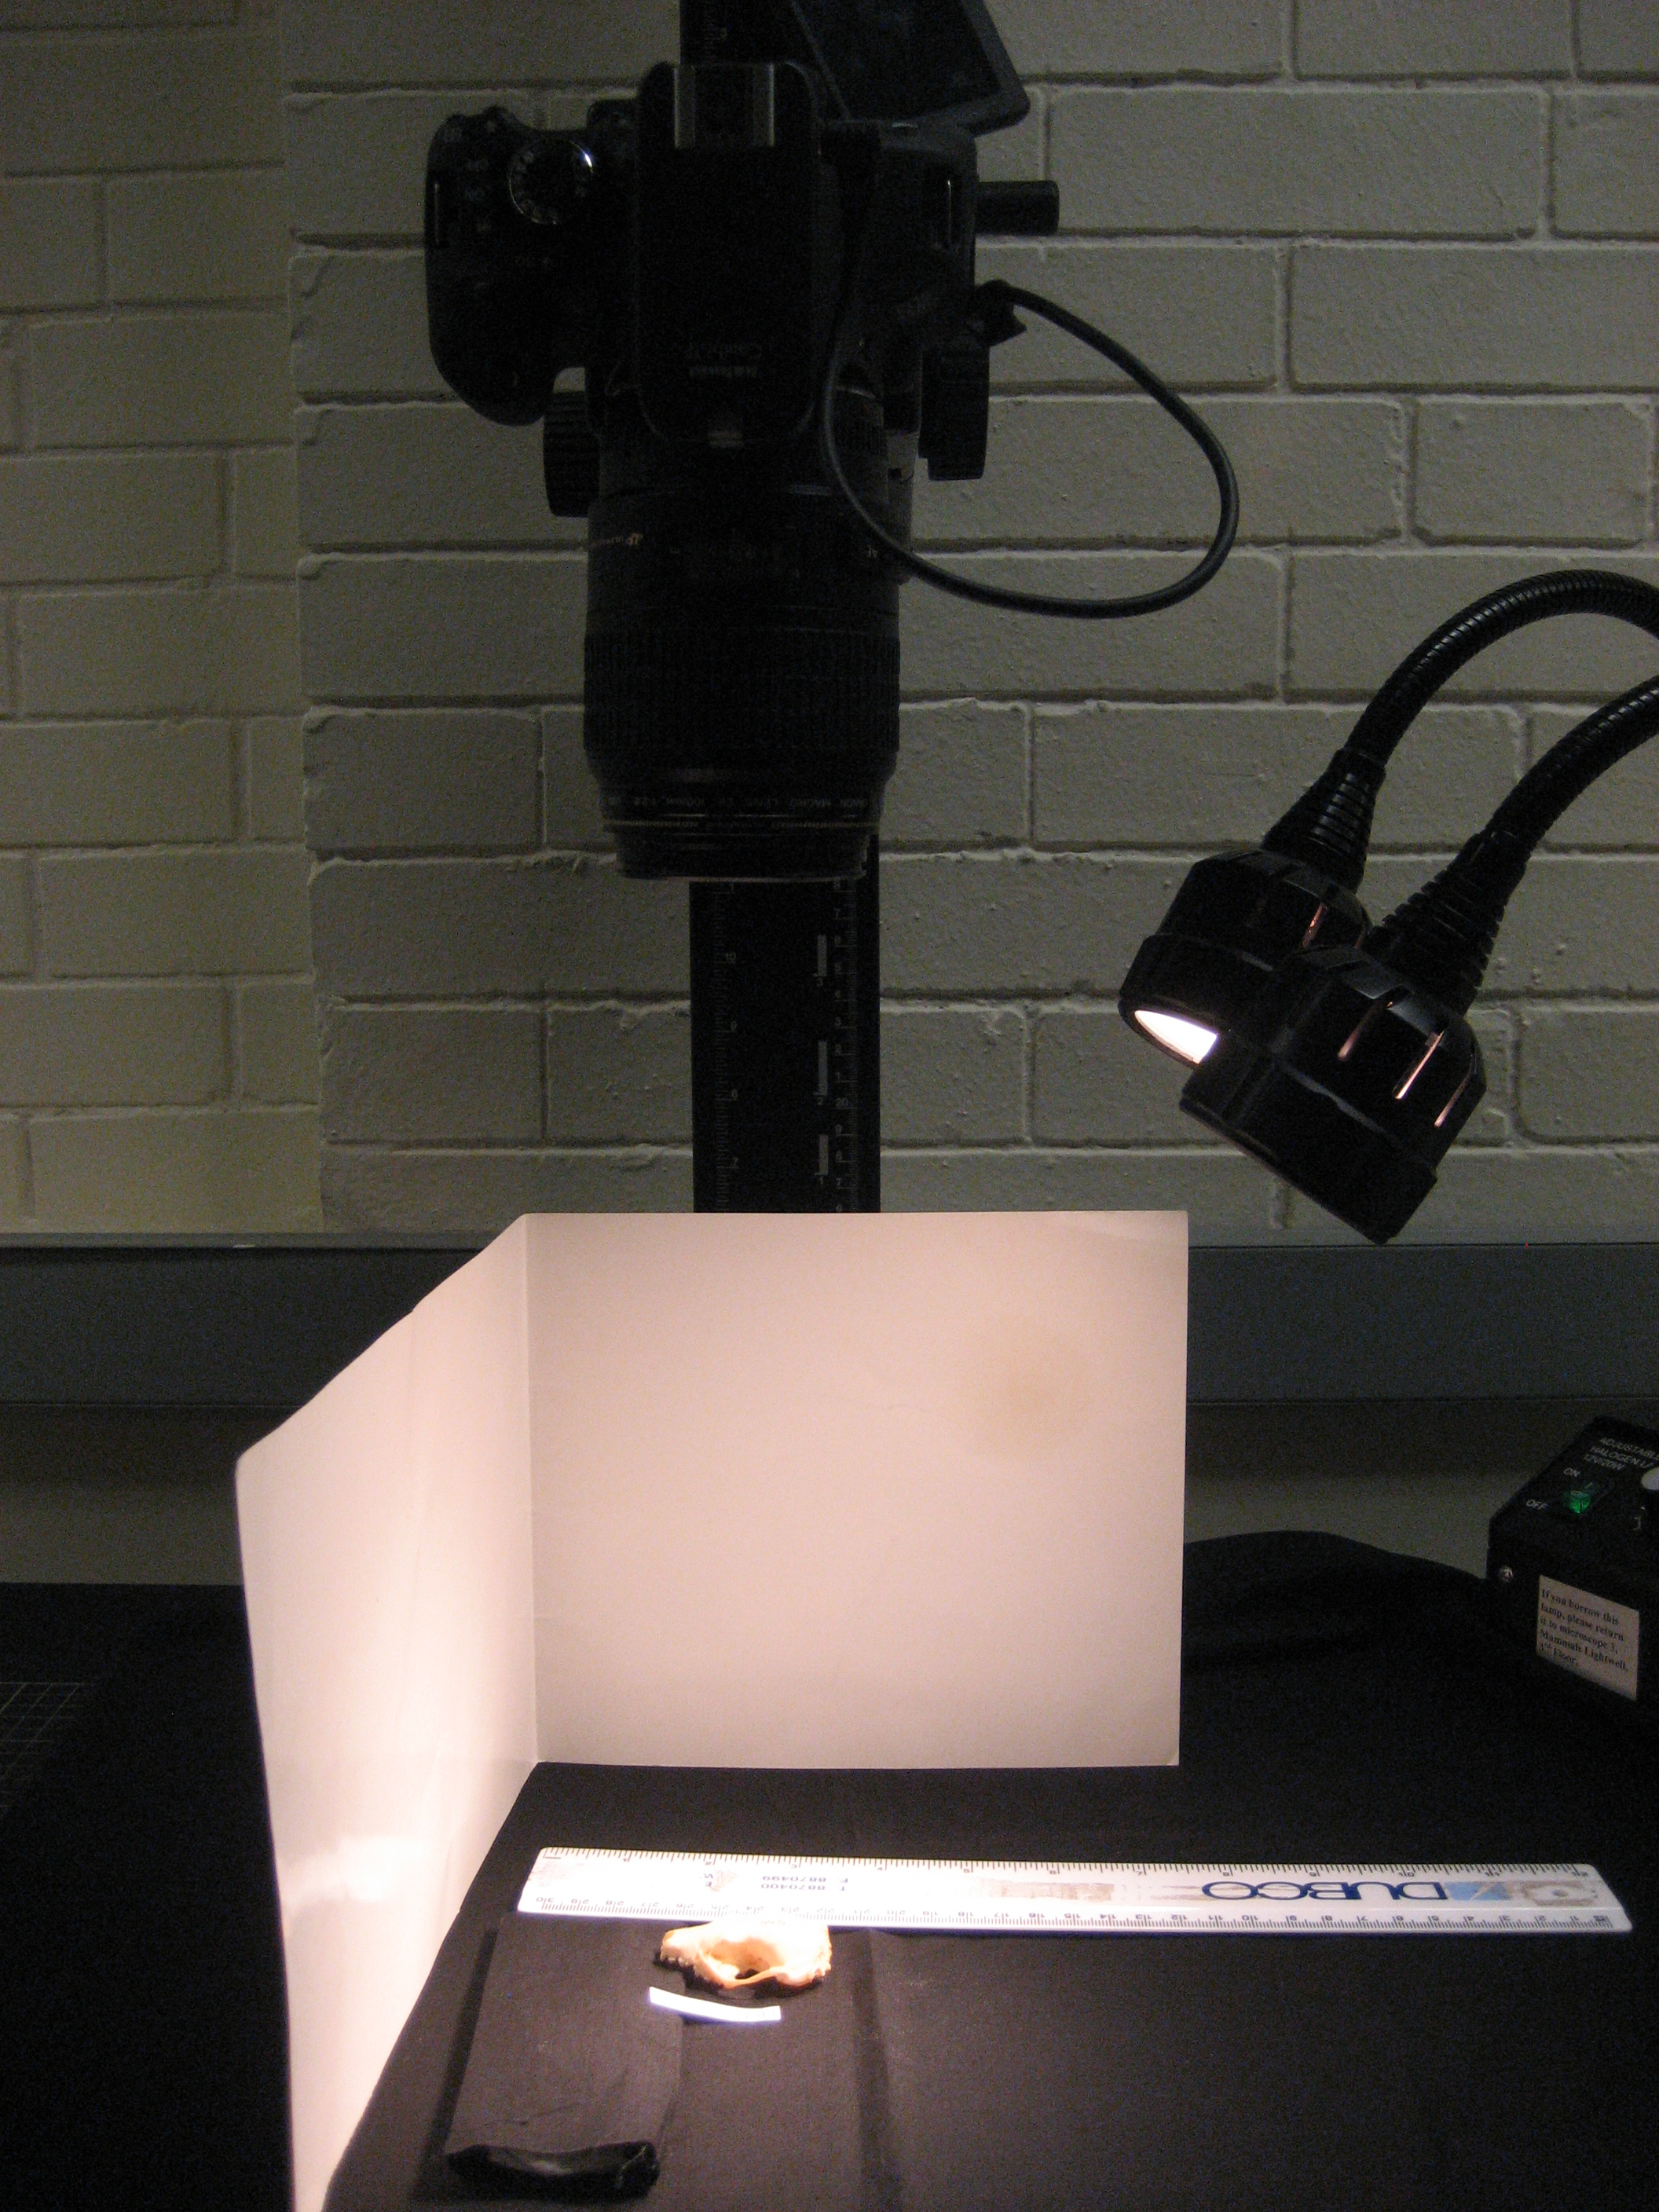
\includegraphics[width=12cm, height=12cm, keepaspectratio=true]{Methods/figures/camera.jpg}
    \caption[Photographic set up]
    {Photographic set up for taking pictures of skulls. The camera (above centre) is fitted to a copy stand, the light source is directed from the top-left corner of the image and the white card reflects the light back onto the skull. }%this is under the figure
  \label{fig:camera}
  \end{figure}
%-------------------------------------------------

\subsection{\normalfont{Photographing specimens}}
	I photographed the skulls in three views; dorsal (top of the cranium), ventral (underside of the skull with the palate roof facing uppermost) and lateral (right side of the skull). I also photographed the outer (buccal) side of the right mandible. When the right sides of either the skull or mandibles were damaged or incomplete I photographed the left sides and later reflected the images so that they could be compared to pictures of the right sides \citep[e.g.][]{Barrow2008}.

% NC: Move to supp mat
	Initially, I tried to take pictures of the limbs in similar orientations to the skulls (dorsal, ventral and lateral). However, there was considerable variation in how the limbs were preserved. For example, some limbs were still articulated while others had fragmented bones. It therefore proved impossible to place the limb bones in consistent orientations that would be comparable across species. Similarly, the small size of some limbs, combined with the frequently incomplete nature of postcranial museum collections, made landmark-based morphometric analyses of any limb pictures impractical. Therefore, I photographed the fore- and hind-limb bones in outer (the side facing away from the rest of the body) and inner (the side facing in towards the centre of the body) views for reference purposes only.

	As I was limited by the maximum camera height available on the copy stands, most skins were too large to be photographed with the 100mm macro lens. Therefore, I used an EFS 18-55mm lens to take pictures of the skins. I photographed skins in the same three orientations as the skulls; dorsal (the upper surface of the animal), ventral (the belly side of the skin) and lateral (right flank of the animal with the skin held in position using bean bags). The dorsal and ventral views give very approximate estimates of the overall body shape of the animal. The lateral views are less biologically relevant since the taxidermic process is unlikely to produce specimens which represent the true body height of the animal.

\subsection{\normalfont{Saving and processing images}}
	Photographs were captured and saved in a raw file format. Before using the pictures for morphometric analyses, I converted the raw files to binary (grey scale) images and re-saved them as TIFF files. The black and white pictures were more useful for later analyses since I was not interested in including any colour comparisons and it is easier to see some biological features in binary images. TIFF files were also appropriate because they are uncompressed (in comparison to JPEG) images and therefore there is less chance of any picture distortions which may affect later analyses \citep{HERC2013}.
	Photographs of the specimens from the American Museum of Natural History and the Smithsonian Institute are available on figshare in separate file sets for the dorsal \citep{Finlay2013d}, ventral \citep{Finlay2013v} and lateral \citep{Finlay2013l} skull pictures along with the mandibles \citep{Finlay2013m}. Copyright restrictions from the other museums prevent public sharing of their images however they are available on request.
	

%##################################################

\section{Geometric morphometric analyses}
\label{sect:morphometrics}

\subsection{\normalfont{Landmark placement on images}}
	%I'm going to have a general "this is morphometrics" overview in my introduction chapter
    %NC: May not really be necessary

	I used a combination of landmark and semilandmark analysis approaches to assess the shape variability in my skull and mandible specimens specimens. 

	I used the TPS software suite \citep{Rohlf2013} to digitise landmarks and curves on my pictures. I set the scale on each pictures individually to standardise for the different camera heights I used when photographing my specimens. I created separate data files for each of my four morphometric analyses (skulls in dorsal, ventral and lateral views and mandibles in lateral view). I digitised landmarks and semilandmark points on every picture individually. Some specimens were too damaged to use so I had a different total number of images for each analysis: skulls dorsal (356), ventral (346), lateral (336) and mandibles (356).
	%Numbers are from the two_family_disparity script after cleaning up the data to remove damages specimens

	When combining landmark and semilandmark approaches, there is a potential problem of over-sampling the curves \citep{MacLeod2012}. To determine the number of semilandmark points required to adequately summarise the curves in my data sets I followed the method outlined by MacLeod \citeyearpar{MacLeod2012}. For each data set I chose a random selection of pictures of specimens which represented the breadth of the morphological data (i.e. specimens from each sub-group of species). I drew the appropriate curves on each specimen and over-sampled the number of points on the curves. I measured the length of the line and regarded that as the 100\%, true length of that outline. I then re-sampled the curves with decreasing numbers of points and measured the length of the outlines. I calculated the length of each re-sampled curve as a percentage of the total length of the curve and then found the average percentage length for that reduced number of semilandmark points across all of the specimens in my test file. I continued this process until I found the minimum number of points that gave a curve length which was at least 95\% accurate.  I repeated these curve-sampling tests for each analysis to determine the minimum number of semilandmark points which would give accurate representations of morphological shape.
	
	Here I summarise the landmarks and curves which I used on each of my different sets of pictures. For landmarks which are defined by dental structures, I used published dental sources \citep{Repenning1967, Eisenberg1969, Nowak1983, MacPhee1987, KnoxJones1992, Davis1997, Querouil2001, Nagorsen2002, Wilson2005, Goodman2006, Karatas2007, Hoffmann2008, Asher2008, Lin2010,  Muldoon2009} where available to identify the number and type of teeth in each species.
	
%------------------------------------------------------------------
\subsection{\normalfont{Skulls: dorsal view}}
	Most of my landmarks in this view are relative (type 3) points which represent overall morphological shape but not necessarily homologous biological features \citep{Zelditch2012}. I placed ten landmarks and drew four semilandmark curves to represent the shape of both the braincase (posterior) and nasal (anterior) area of the skulls (figure \ref{fig:skdors_skvent}). Table \ref{tab:skdors} describes how I placed the landmarks and drew the outline curves for my dorsal skull pictures 

\subsection{\normalfont{Skulls: ventral view}}

	Most of the landmarks in this view are concentrated around the dentition and palate of the animals. I placed 13 landmarks and drew one outline curve (resampled to 60 semilandmark points) around the back of the skull between landmarks 12 and 13 (figure \ref{fig:skdors_skvent}). The high variability of my species' basi-cranial region and difficulties associated with identifying developmentally or functionally homologous points precluded designation of additional landmarks towards the back of the skulls. Table \ref{tab:skvent} outlines the descriptions of the landmarks I placed on the ventral pictures.

%------------------------------------------------
%Change to having combined pictures of skulls and mandibles
%I re-did them compared to the disparity manuscript to be in black and white

%Skulls dorsal and ventral

\begin{figure}[!htbp]
	\centering
	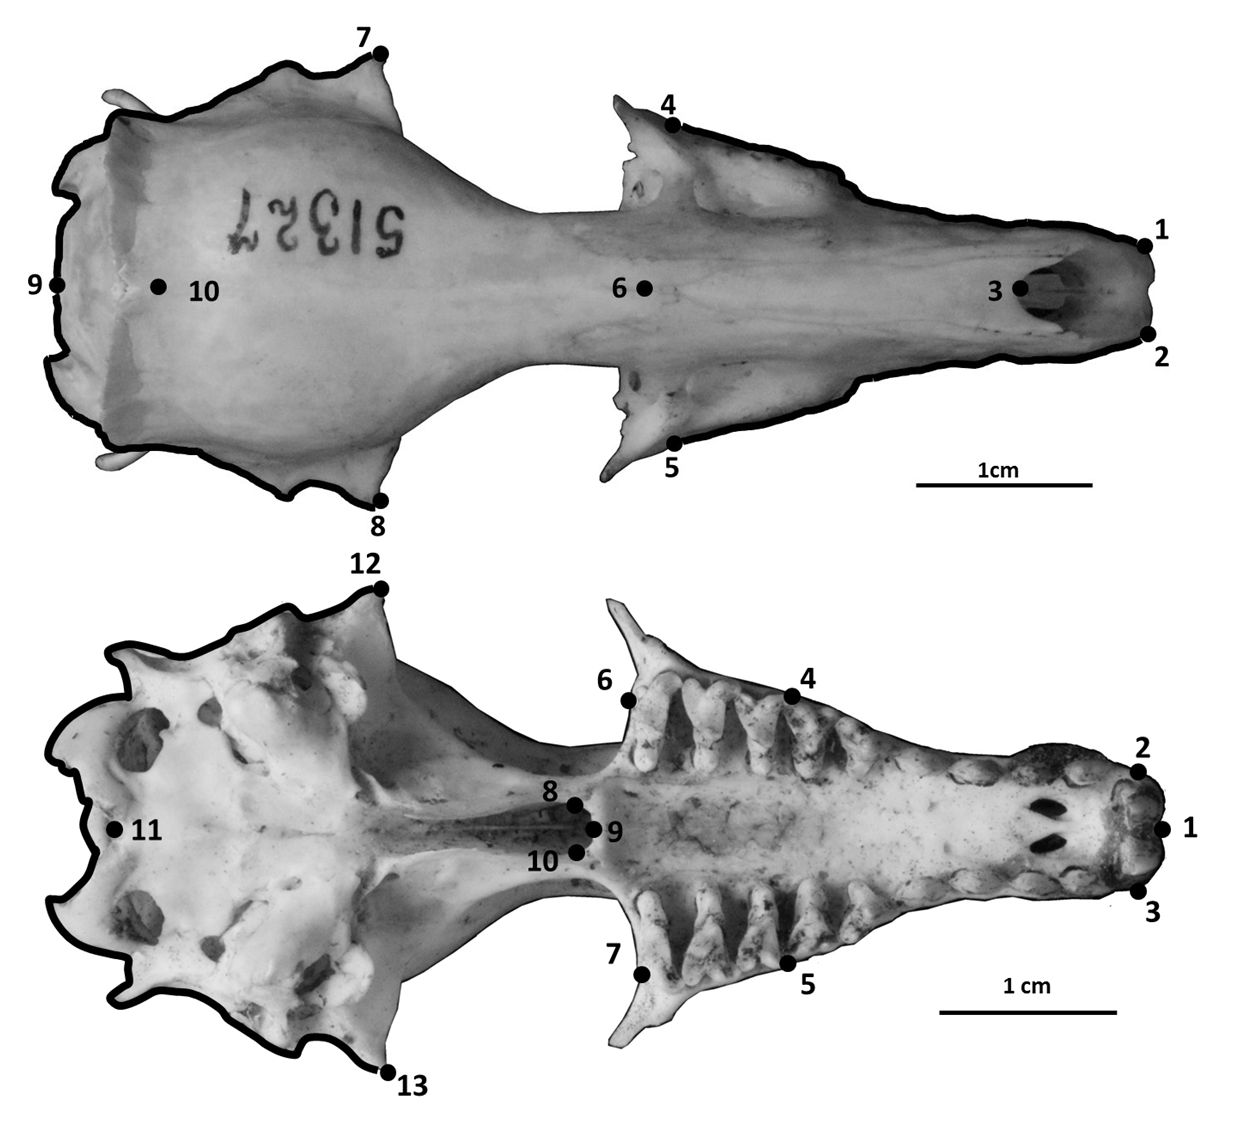
\includegraphics[width=1\linewidth]{Methods/figures/Skdors+Skvent_combined_BW.png}
	\caption[Skulls: dorsal and ventral landmarks]
	{Landmarks (numbered points) and curves(outlines) for the skulls in dorsal and ventral view. See tables \ref{tab:skdors} and \ref{tab:skvent} for landmark descriptions. The skulls are two different specimens of \textit{Potamogale velox} (otter shrew tenrec), museum accession numbers AMNH 51327 and BMNH 1934.6.16.2. }
	\label{fig:skdors_skvent}
\end{figure}


%Skdors descriptions

\begin{table}[h]
	\caption[Skulls: dorsal landmarks]
		{Descriptions of the landmarks (points) and curves (semilandmarks) for the skulls in dorsal view (figure
		\ref{fig:skdors_skvent})} 
	%Skdors landmarks

\begin{tabular}[t]{p{3cm}  l}		
\hline
\textbf{Landmark} & \textbf{Description} \\
\hline
%------------------------------------------------------------
1 + 2 & Left (1) and right (2) anterior points of the premaxilla \\
%------------------------------------------------------------
3 & Anterior of the nasal bones in the midline \\
%------------------------------------------------------------
4 + 5 &	Maximum width of the palate (maxillary) on the left (4) and right (5)\\
%------------------------------------------------------------
6 & Midline intersection between nasal and frontal bones \\
%------------------------------------------------------------
7 + 8 & Widest point of the skull on the left (7) and right (8) \\
%------------------------------------------------------------
9 &	Posterior of the skull in the midline \\
	%Panchetti 2008 and Macholan2008 have different definitions for this one so I need to choose one
%------------------------------------------------------------
10 & Posterior intersection between saggital and parietal sutures \\
%--------------------------------------
\hline
\textbf{Curve A} & Outline of the braincase on the left side, between landmarks 9 and 7\\ 
(12 points) & (does not include visible features from the lower (ventral) side of the skull) \\

\textbf{Curve B} & Outline of the palate on the left side, between landamarks 4 and 1 \\
(10 points) & (outline of the rostrum only, not the shape of the teeth)\\

\textbf{Curve C} &	Outline of the braincase on the right side, between landmarks 9 and 8 \\
(12 points) & (does not include visible features from the lower (ventral) side of the skull) \\

\textbf{Curve D} & Outline of the palate on the right side, between landamarks 5 and 2 \\
(10 points) & (outline of the rostrum only, not the shape of the teeth)\\
%------------------------------------------------------------
\hline
\end{tabular}
	\label{tab:skdors}
\end{table}

%Skvent descriptions
\begin{table}[!htb] %force the table to go up with the picture
\caption[Skulls: ventral landmarks]
		{Descriptions of the landmarks (points) and curves (semilandmarks) for the skulls in ventral view (figure \ref{fig:skdors_skvent}).} 
%SkVent landmarks
\begin{tabular}[t]{p{0.2\textwidth} p{0.75\textwidth}}		
\hline
\textbf{Landmark} & \textbf{Description} \\
\hline
%--------------------------------------
1 & Anterior point of the palate\\
%--------------------------------------
2 + 3 & Posterior, lateral extremity of the right (2) and left (3) incisor\\
%--------------------------------------
4 + 5 & Anterior, outer point of the first molar on the right (4) and left (5)\\
%--------------------------------------
6 + 7 & Posterior, outermost point of the last molar surface on the right (6) and left (7) \\
%--------------------------------------
8 & Widest point of the curve of the palatine on the right side\\
%--------------------------------------
9 & Posterior point of the palatine in the midline\\
%--------------------------------------
10 & Widest point of the curve of the palatine on the left side\\
%--------------------------------------
11 & Anterior of the occipital foramen in the midline\\
%--------------------------------------
12 + 13 & Widest (extreme lateral) point of the braincase on the right (12) and left (13)\\
%--------------------------------------
Curve*  & Outline of the back of the skull (between landmarks 12 and 13), 60 points \\
%------------------------------------------------------------
\hline
\end{tabular}
\label{tab:skvent}
\end{table}
%-------------------------------------------------------------
\newpage
\subsection{\normalfont{Skulls: lateral view}}
	I placed nine landmarks on the lateral pictures (figure \ref{fig:sklat_mands}) and also drew two semilandmark curves between landmarks 7 and 8 to represent the shape of the back of the skull (resampled to 20 semilandmark points) and landmarks 8 and 1 (resampled to 15 semilandmark points) down the midline of the nose to represent the shape of the top of the skull. Table \ref{tab:sklat} describes my definitions for each of the landmark points.
	If specimens were damaged on their right side I reflected photographs of the left lateral side of the skull so that all pictures would be in the same orientation.
	I originally tried to include more landmarks around the infraorbital foramina (IF) as a crude measure of facial sensitivity and because the IF area is correlated with ecotypes \citep{Crumpton2012}. However, it proved impossible to see the boundaries of the IF in many species and single landmark points could not represent the shape of the full foramina. 
% NC: So did you include these or not? If not don't mention it.

\subsection{\normalfont{Mandibles}}
	I placed seven landmarks and drew four curves on each mandible picture (again, reflecting any pictures of the left mandible so they could be compared to pictures of the right side, figure \ref{fig:sklat_mands}). I drew separate curves around each of the three processes of the ascending ramus: coronoid, condyloid and angular and along the base of the horizontal ramus of the jaw. While obviously part of an integrated jaw unit, the development of the mandibular processes are also, in some aspects, independent since they attach different muscles which exert different masticatory forces on the jaw \citep{Barrow2008}. Therefore, by drawing separate curves around each of these elements, my analyses could assess the relative shape changes of different components of the jaw with relevance to variation in feeding strategies and capabilities.

%********
%Why do we care about independence??
%I don’t like how I’ve phrased the above paragraph but I just thought it was a nice point in the Barrow paper so I want to include it somewhere.
% NC: It's nice yes, but is it relevant? Or necessary?
%********

%---------------------------------------------------
%Combined sklat and mandibles diagrams


\begin{figure}[!htbp]
	\centering
	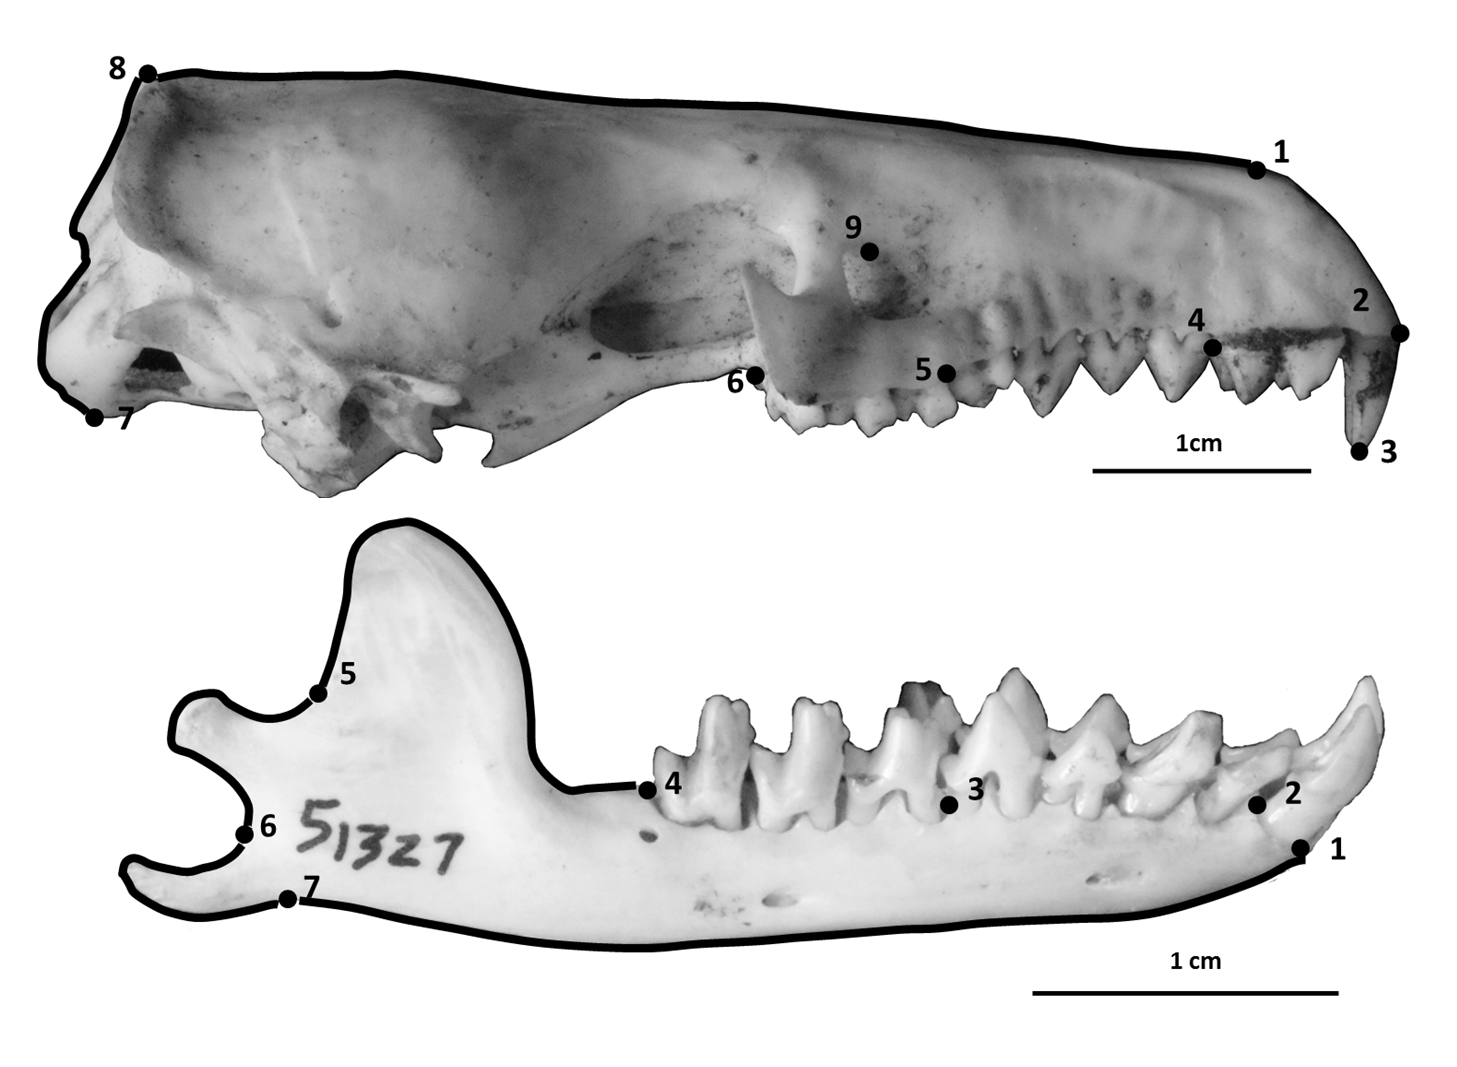
\includegraphics[width=1\linewidth]{Methods/figures/Sklat+mands_combined_BW.png}
	\caption[Lateral skulls and mandibles landmarks]
	{Landmarks (numbered points) and curves(outlines) for the skulls and mandibles in lateral view. See tables \ref{tab:sklat} and \ref{tab:mands} for landmark descriptions. The skull (BMNH 1934.6.16.2.) and mandible (AMNH 51327) belong to two different specimens of \textit{Potamogale velox} (otter shrew tenrec).}
	\label{fig:sklat_mands}
\end{figure}

%Sklat descriptions

\begin{table}[!htb]
\caption[Skulls: lateral landmarks]
		{Descriptions of the landmarks (points) and curves (semilandmarks) for the skulls in lateral view (figure \ref{fig:sklat_mands}).} 
%Sklat landmarks

\begin{tabular}[t]{p{2cm} p{12cm}}		
\hline
\textbf{Landmark} & \textbf{Description} \\
\hline
%--------------------------------------
1 & Anterior, upper tip of the nasal bone\\
%--------------------------------------
2 & Anterior of the alveolus of the first incisor\\
%--------------------------------------
3 & Lowest point of the first incisor\\
%--------------------------------------
4& Posterior of the alveolus of the last incisor \\
%--------------------------------------
5 & Anterior tip of the alveolus of the first molar\\
%--------------------------------------
6 & Posterior tip of the alveolus of the last molar\\
%--------------------------------------
7 & Lowest point of the basi-occipital (base of the back of the skull)\\
%--------------------------------------
8 & Highest point of the braincase\\
%--------------------------------------
9 & Highest point of the infraorbital foramen\\
%--------------------------------------
\hline
\textbf{Curve A} & Between points 7 and 8  \\
(20 points)& Back of the skull from the lowest to highest points\\
%------------------------------------------------------------
\textbf{Curve B} & Between points 8 and 1  \\
(15 points)&From the highest point of the braincase to the front of the nasal \\
%------------------------------------------------------------
\hline
\end{tabular}
\label{tab:sklat}
\end{table}

\begin{table}[!htb]			
	\centering
	\caption[Mandibles: landmarks]
		{Descriptions of the landmarks (points) and curves (semilandmarks) for the mandibles in lateral (buccal) view (figure \ref{fig:sklat_mands}).}
	%Mandibles landmarks


\begin{tabular}[t]{p{0.2\textwidth} p{0.75\textwidth}}		
\hline
\textbf{Landmark} & \textbf{Description} \\
\hline
1 & Anterior of the alveolus of the first incisor \\
2 & Posterior of the alveolus of the first incisor \\
3 &	Anterior of the alveolus of the first molar \\
4 & Posterior of the alveolus of the last molar \\
5 & Maximum curvature between the coronoid and condylar processes\\
6 & Maximum curvature between the condylar and angular processes  \\
7 &	Maximum curvature between the angular process and the horizontal ramus \\
%---------------------------------------------------
\hline
Curve A & Condyloid process (between landmarks 4 and 5, 15 points)\\
Curve B & Condylar process (between landmarks 5 and 6, 15 points) \\
Curve C & Angular process (between landmarks 6 and 7, 15 points)  \\
Curve D & Base of the jaw (between landmarks 7 and 1, 12 points)  \\
%---------------------------------------------------
\hline
\end{tabular}
	\label{tab:mands} 
\end{table}




%-----------------------------------------------

\subsection{\normalfont{Procrustes superimposition}}
\label{sect:procrustes}

	After creating my files with the landmarks and semilandmarks placed on each picture, I used TPSUtil \citep{Rohlf2012} to create "sliders" files that defined which points in the TPS files should be treated as semilandmarks \citep{Zelditch2012}. I conducted all further morphometric analyses in R version 3.0.2 \citep{Team2014} within the geomorph package \citep{Adams2013}.
	
	% NC: Not needed - of course you'd do it for every picture. And you can discuss the extra uses of the data in the discussion
	%I placed landmarks and semilandmarks on all the pictures from every specimen. However, for the purposes of comparing morphological diversity in tenrecs to their closest relatives (chapter \ref{chap:disparity} I only used the tenrec and golden mole subset of the data. However, the TPS files containing landmark coordinates for all remaining species could be used for future analyses of morphological convergence (see discussion in chapter \ref{chap:discussion}). 
	
	I used the gpagen function in the geomorph package \citep{Adams2013} to run a general Procrustes alignment \citep{Rohlf1993} of the landmark coordinates while sliding the semilandmarks by minimising Procrustes distance \citep{Bookstein1997}.
	I used these Procrustes-aligned coordinates of all specimens to calculate average shape values for each species which I then used for a principal components (PC) analysis with the plotTangentSpace function \citep{Adams2013}. 
	

%####################################################

%I'm not sure whether this is the most appropriate way to deal with errors: I could split up the sections and put them at the end of each of the previous sections rather than breaking up the story here but that might be more fragmented overall

% NC: I think this can probably be reintegrated mostly with the rest of the section. Only 5 is really relevant. So maybe just have a section on "Potential morphometrics errors" rather than error checking? Or add as a subsection to the 2D data collection?

\section{Error checking}
\label{sect:errors}
	My data are prone to a number of different sources of error. These include 1) taxonomic identification which has not been updated to currently accepted names, 2) specimen identification errors, 3) possible variation associated with sex and age class of individuals, 4) the accuracy and repeatability with which species traits are measured, 5) morphometric errors associated with photographing specimens and the placement of landmarks. I address each of these possible sources of error below.  

\subsection{\normalfont{Taxonomic}}
	I recorded species names as they were written on museum specimen labels and then corrected them to match the taxonomy in Wilson and Reeder's Mammal Species of the World \citeyearpar{Wilson2005}. For recently identified species, such as \textit{Microgale jobihely} \citep{Goodman2006}, which are not included in Wilson and Reeder \citeyearpar{Wilson2005}, I used the taxonomy recorded on the labels. 
	% NC: Haven't you already said this in data collection above? Maybe just pop it in the relevant place?

\subsection{\normalfont{Specimen identification}}
	%add in Natalie's centroid means?
	% NC: So this is only an issue for these four? If so maybe pop into supp material as you don't use them
	
	There were four specimens from the Smithsonian Institute that had species labels which did not match between skulls and skins with the same specimen ID numbers. The four skulls were labeled as \textit{Hemicentetes semispinosus}. The corresponding skins were originally labeled as \textit{H. semispinosus} but this was crossed out and changed to \textit{H. nigriceps}. The re-labeled skins looked clearly different to the undisputed \textit{H. semispinosus} skins and also look more similar to other pictures of \textit{H. nigriceps}. Therefore, I made the assumption that the re-labeling of the skins as \textit{H. nigriceps} represents the true taxonomy and I treated the corresponding skulls as \textit{H. nigriceps}.

\subsection{\normalfont{Specimen sex and age}}
% NC: could just mention this when talking about how you selected specimens to measure since you don't actually quantify or fix the error.

	Age classification of mammal skulls is usually based on dental characteristics and cranial fusion.
 	However, it is difficult to age-classify tenrecs in this way. In some species the last molar does not erupt fully until the first molar has been shed so the full dentition is never present at any one time \citep{Nowak1983}. Furthermore, it is difficult to distinguish deciduous from permanent teeth in \textit{Microgale} tenrecs \citep{Asher2008} which has led to confusion and misidentification of juvenile forms as separate species \citep{Olson2004}.
 	I identified and excluded any obviously juvenile specimens based on incomplete cranial fusion. When specimens could not be obviously identified as juveniles I treated them all as equivalent adult forms. 	
	I included both male and female specimens in my data as I am interested in cranial shape of the species as a whole regardless of whether or not there are differences due to sexual size dimorphism.


\subsection{\normalfont{Linear measurements}}
	%Maybe this isn't relevant anymore since I'm not actually doing anything with the linear measurement data?
	%I've kept it in for the moment as a reference incase anyone wants to use the data in the future
	% NC: Yeah I'd pop this into the supp material
	
	As mentioned above (section \ref{sect:measurements}), I took three replicate measurements of most of my variables and five replicates of other, smaller variables. 
	Some morphometric studies take replicate measurements of a trait and use the average value for further analyses (REFS?). Rather than taking the mean of each of three (or five) measures, I used the median as it is less likely to be skewed by outliers and gives a more accurate representation of the true value of the trait (REFS?).
	
	%Come back to here for references
	
	Before extracting the median values, I followed the protocol for assessing measurement error outlined by \citep{Cooper2009}. This method assesses whether there is a reasonable correlation among the replicate measurements of the same variable. The error checking criteria are based on two calculations; the coefficient of variation and the percentage spread.
	
	I calculated the coefficient of variation (standard deviation/mean*100) for each measurement. This value estimates the extent to which replicate measurements deviate from the mean. When the coefficient of variation was less than 5\%, I accepted the median value as an accurate measurement of the size of the structure. 
	If the coefficient of variation was greater than 5\%, indicative of a low agreement between replicate measurements, I measured the percentage spread of the data. For variables measured three times, I calculated percentage spread as [(minimum difference between neighbouring measurements)/ (range of measured values)*100].
	For variables that I measured five times, the differences between neighbouring values were calculated and labelled from smallest to largest as a, b, c, and d with the range of the measured values designated as e \citep{Cooper2009}. For these variables, I calculated percentage spread as [(a/e + b/e + c/e)*100]. 
	Small percentage spread values indicate close agreement between repeated measurements. When percentage spread approaches 50\% the data are evenly spread out and therefore there is no way of knowing whether the median value is an accurate measurement of the trait \citep{Cooper2009}. I chose to use to use 25\% as a cut off point for accepting the accuracy of measured traits.

	I used these error checking criteria to assess the accuracy of my repeated measurements of both skulls and limbs. 

%I've taken this out for now since I'm not actually using any of the linear measurement data
	%Of the 20 measurements for xxx skulls, there were xx variables belonging to xx skulls which had coefficient of variation > 5\% and percentage spread >25 \%. My final skull data set included xx replicates of xx variables from xx specimens comprising xx species.

	%Of the 19 measurements for xxx limbs, there were xx variables belonging to xx specimens which had coefficient of variation > 5\% and percentage spread >25 \%. My final limb data set included xx replicates of xx variables from xx specimens comprising xx species.

\subsection{\normalfont{Potential morphometrics errors}}

    % NC: Not relevant
	%I used 2D morphometrics to compare the morphologies of the skulls (section \ref{sect:morphometrics}). The small size of my specimens, combined with the number of specimens involved in my study made 3D imaging impractical. It takes roughly 1.5 hours for a good quality scan of each specimen so it would have taken me at least 550 hours to scan the 366 specimens that I photographed.
	 
	While 2D methods are an accepted means of comparing morphological shape \citep[e.g.][]{Adams2004, Mitteroecker2009}, particularly for comparing skull morphologies of small mammals \citep[e.g.][]{Cardini2003, Panchetti2008, White2008, Barrow2008, Scalici2011}, the inherent discrepancies associated with comparing three dimensional objects using two dimensional pictures can introduce some potential problems of possible image distortion \citep{Arnqvist1998}. Similarly, human error with how landmarks are positioned on specimens could also introduce noise into further analyses. 
	
	In contrast to detailed intraspecific work \citep[e.g.][]{Bornholdt2008, Blagojevic2011} photographic or landmark placement errors are unlikely to be significant in my interspecific study since one would expect that the morphological variation among species is large enough to  be detected as a signal above any background noise associated with methodological error \citep{Arnqvist1998}. Nevertheless, it is still important to assess measurement error in a morphometric data set to increase confidence in the outcome of final analyses.
	I identify two main sources of morphometric measurement error; specimen orientation and placement of landmarks.

	Variation in the orientation of specimens for photography is one of the main sources of error in 2D morphometric studies \citep{Adriaens2007}. If specimens are not placed on a flat plane or in a consistent position relative to the camera, areas of the object which are tilted towards the camera will appear to be larger than reality, distorting any subsequent morphometric analyses of the shape. 
	I placed the landmarks on each set of pictures so inter-observer variation in landmark placement is not an issue for my study.  However, repeatability and reliability of my choice of landmarks could affect the final results of my analyses \citep{Arnqvist1998}.
	%Need to fix this reference: it's okay in the bibliography but it doesn't all show up here

	To measure potential orientation error, I photographed the skulls (dorsal, ventral and lateral views) and mandibles of each specimen three times, cycling through the pictures so that the specimen was removed and re-positioned before every shot \citep{Viscosi2011}.
	I used a subset of my ventral skull pictures to test for two sources of error: specimen orientation and landmark placement error \citep{Arnqvist1998, Barrow2008}. Of the specimens which I photographed three times,  I chose a random subset of seven skulls from four different Families: three tenrecs and single representatives of shrews, moles, hedgehogs and golden moles. I copied these images and placed landmarks on three copies of each image to compare variation in landmark placement within each orientation (three copies of the one image). This gave nine replicates of each skull: three separate pictures, and three copies of each of those pictures. As before, I ran a general Procrustes alignment \citep{Rohlf1993} of the specimens, calculated the average shape values for each skull (average of all nine pictures) and used these values for a principal components (PC) analysis. 
		
	I used a linear mixed effects model to model the shape variation (first PC axis) associated with specimen (fixed effect) and two nested random effects: picture identity nested within specimen and picture replicate nested within picture. I ran the test using the lmer function in the lme4 package \citep{Bates2014}. % NC: Need to explain more clearly what you mean here. Why the nesting? What would a sig result show you?

	Specimen orientation and landmark placement had negligible effects on the overall shape variation between different skulls (2.76 x 10\textsuperscript{-16} $\pm$ 1.66 x 10\textsuperscript{-8} and 7.4 x 10\textsuperscript{-14} $\pm$ 2.72 x 10\textsuperscript{-7} respectively). % NC: What are these numbers? Estimates? Effect sizes?
	
	Therefore, I am confident that shape variation between the specimens in the rest of my analyses reflected true morphological differences rather than methodological error.
%----------------------------------------------------
%Do I need a summary at the end to tie into the next chapter?

% NC: Nope!






